\chapter{Electrostatics}

\modinfo{Directory}{Electrostatics}
\modinfo{Solvers}{\Idx{StatElecSolve}, \Idx{ElectricForce}}
\modinfo{Tools}{\Idx{ElmerGrid}, editor}
\modinfo{Dimensions}{3D, Steady-state}

\subsection*{Case definition}

This case presents solving the Poisson equation for electric potential
and calculating appropriate derived quantities, such as
\Idx{capacitance}, based on the result. The geometry studied is a
symmetric quadrant of a plane capacitor having a rectangular hole in
another plate. A setting of this kind can be used to study the effects
of geometrical features on the capacitance and on the electrostatic
force, which both are meaningful quantities for coupled
simulations in {\em e.g.}  microsystems.


\subsection*{Solution procedure}

The mesh is constructed using ElmerGrid with the following command
\ttbegin
ElmerGrid 1 2 elmesh.grd
\ttend
The mesh is extended above the hole to avoid undesired boundary
effects. The geometry is presented in the Figure~\ref{geo_elstat}

\begin{figure}[hbt]
  \centerline{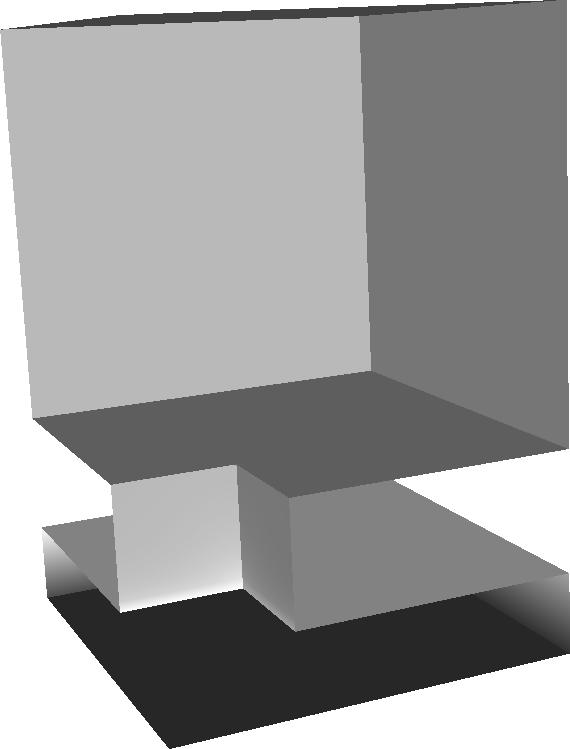
\includegraphics[width=0.32\textwidth]{geo_elstat}}
  \caption{The geometry of problem.} 
  \label{geo_elstat}
\end{figure}

The simulation problem includes a single body, and thus one material
and one equation set, as well as three solvers. The solvers are used
to compute the electric potential and related quantities, to calculate
the electric force, and to save relevant data into a file. This
tutorial is defined in Elmer \Idx{MEMS} units. The sif-file is presented
below.

\ttbegin
Check Keywords Warn

Header
  Mesh DB "." "elmesh"
End
\ttend

Only a single steady state iteration is needed, since the Poisson
equation is linear.
\ttbegin
Simulation
  Coordinate System = Cartesian 3D
  Simulation Type = Steady State
  Steady State Max Iterations = 1
  Output File = "elstatics.result"
  Post File = "elstatics.vtu"
End
\ttend

The permittivity of vacuum has to be defined in the Constants section.
\ttbegin
Constants
  Permittivity Of Vacuum = 8.8542e-12
End

Body 1
  Equation = 1
  Material = 1
End
\ttend

Electric energy density is added into the results in Equation
section. This allows energy density to be visualised.
Here the visualization is done with now obsolete ElmerPost
but you would probably rather use Paraview (or some other software that
can handle VTU files). 
Note also, that calculating electric flux (or the electric
displacement field) is disabled in the Solver~1 block. Further, the
potential difference used in calculating the capacitance of the system
has to be defined in this section. This should be the same as the
boundary conditions define for the capacitance calculation to be
sensible.
\ttbegin
Equation 1
  Active Solvers(2) = 1 2
  Calculate Electric Energy = True  ! (default False)
End

Solver 1
  Equation = Stat Elec Solver
  Variable = Potential
  Variable DOFs = 1
  Procedure = "StatElecSolve" "StatElecSolver"
  Calculate Electric Field = True  ! (default True)
  Calculate Electric Flux = False  ! (default True)
  Potential Difference = 1.0e6
  Linear System Solver = Iterative
  Linear System Iterative Method = BiCGStab
  Linear System Max Iterations = 200
  Linear System Convergence Tolerance = 1.0e-07
  Linear System Preconditioning = ILU1
  Linear System ILUT Tolerance = 1.0e-03
  Nonlinear System Max Iterations = 1
  Nonlinear System Convergence Tolerance = 1.0e-4
  Nonlinear System Newton After Tolerance = 1.0e-3
  Nonlinear System Newton After Iterations = 10
  Nonlinear System Relaxation Factor = 1
  Steady State Convergence Tolerance = 1.0e-4
End
\ttend

The static electric force solver does not need a lot of information:
\ttbegin
Solver 2
  Equation = Electric Force
  Procedure = "ElectricForce" "StatElecForce"
End
\ttend

Finally, some data is saved in file scalars.dat in working directory.
\ttbegin
Solver 3
  Exec Solver = After All
  Equation = SaveScalars
  Procedure = "\Idx{SaveData}" "SaveScalars"
  Filename = "scalars.dat"
End
\ttend

Only the relative permittivity of the material has to be defined.
\ttbegin
Material 1
  Relative Permittivity = 1
End
\ttend

The boundary conditions include the values of electric potential
(voltage) and indication on which boundary the electric force should
be calculated. On all the other boundaries a natural boundary
condition is used, basically stating that the electric flux through
these boundaries is zero.
\ttbegin
Boundary Condition 1
  Target Boundaries = 4
  Potential = 0.0
  Calculate Electric Force = True
End

Boundary Condition 2
  Target Boundaries = 3
  Potential = 1.0e6
End
\ttend


\subsection*{Results}

The results obtained for capacitance and electric force are compared
to those of a complete plane capacitor. For a plane capacitor, the
capacitance is
\begin{equation}
C=\varepsilon_r\varepsilon_0\frac{A}{d},
\end{equation}
and the electrostatic force is
\begin{equation}
F_e = \frac{1}{2}\varepsilon_r\varepsilon_0\frac{A}{d^2}\Phi^2,
\end{equation}
where $\varepsilon_r$ is the relative permittivity, $\varepsilon_0$
is the permittivity of vacuum, $A$ is the area of a capacitor plate,
$d$ is the separation of the capacitor plates, and $\Phi$ is the
potential difference between the plates.

The results of the simulation as well as the comparison to the
complete plane capacitor values are shown in Table~\ref{tab_elstatics}
(in Elmer MEMS units). Note that the fringe fields on capacitor edges
are not calculated. This would require much larger mesh extending
outside the capacitor boundaries.

\begin{table}[htb]
\caption{Comparison of numerical results to analytic values}
\label{tab_elstatics}
\begin{center}
\begin{tabular}{lccc} \hline
            & simulation & analytic & ratio \\ \hline
Capacitance & \ \ $2.1361\cdot 10^{-10}$\ \  & 
              \ \ $2.2136\cdot 10^{-10}$\ \  & 0.965 \\
Electric Force & $1.0406\cdot 10^2$ & 
                 $1.1068\cdot 10^2$ & 0.940 \\ \hline
\end{tabular}
\end{center}
\end{table}

Finally, a picture of the results is presented. The
Figure~\ref{res_elstat} shows the isosurfaces of the electric
potential with the color marking the strength of the electric
field. From the picture it is clearly seen that the electric field is
constant between the plates except for the proximity of the hole which
causes weakening of the field magnitude. There are also strong
electric fields at the edges of the hole.


\begin{figure}[hbt]
  \centerline{
\includegraphics[width=0.8\textwidth]{res_elstat}}
  \caption{Isosurfaces of the potential coloured with electric field
  magnitude.} 
  \label{res_elstat}
\end{figure}



\vfill
\mbox{}

